\chapter{Opis projektnog zadatka}
		
		\textbf{\textit{dio 1. revizije}}\\
		
		\textit{Na osnovi projektnog zadatka detaljno opisati korisničke zahtjeve. Što jasnije opisati cilj projektnog zadatka, razraditi problematiku zadatka, dodati nove aspekte problema i potencijalnih rješenja. Očekuje se minimalno 3, a poželjno 4-5 stranica opisa.	Teme koje treba dodatno razraditi u ovom poglavlju su:}
		\begin{packed_item}
			\item \textit{potencijalna korist ovog projekta}
			\item \textit{postojeća slična rješenja (istražiti i ukratko opisati razlike u odnosu na zadani zadatak). Dodajte slike koja predočavaju slična rješenja.}
			\item \textit{skup korisnika koji bi mogao biti zainteresiran za ostvareno rješenje.}
			\item \textit{mogućnost prilagodbe rješenja }
			\item \textit{opseg projektnog zadatka}
			\item \textit{moguće nadogradnje projektnog zadatka}
		\end{packed_item}
		
		\textit{Za pomoć pogledati reference navedene u poglavlju „Popis literature“, a po potrebi konzultirati sadržaj na internetu koji nudi dobre smjernice u tom pogledu.}
		\eject
		
		
		Cilj ovog zadatka je napraviti aplikacijsko programsko sučelje koje će olakšati komunikaciju između istraživača, voditelja postaja te tragača u akcijama praćenja divljih životinja.
		
		Prvi korak za korištenje aplikacije je registracija. Prilikom registracije korisnik odabire koju bi ulogu imao u aplikaciji. To može biti istraživač, voditelj postaje ili tragač.
		Podaci koje je potrebno unijeti pri registraciji su sljedeći:
		\begin{packed_item}
			\item \textit{korisničko ime}
			\item \textit{fotografija}
			\item \textit{lozinka}
			\item \textit{ime}
			\item \textit{prezime}
			\item \textit{email adresa.}
		\end{packed_item}
		
		Registracija završava potvrdom preko emaila, te dodatno voditelja i istraživača treba potvrditi administrator. Sličan primjer obrasca za registraciju prikazan je u nastavku na slici 1.
		Voditelj ima svoju postaju koja ima naziv po području na kojem se nalazi (npr. Kopački rit, Velebit…). Također posjeduje popis tragača koji su dio njegove postaje te na koji način mogu obavljati istraživanje. Mogućnosti kretanja tragača su sljedeće:
		\begin{packed_item}
			\item \textit{pješke}
			\item \textit{automobilom}
			\item \textit{cross motorom}
			\item \textit{brodom}
			\item \textit{dronom}
			\item \textit{helikopterom.}
		\end{packed_item}
		
		Akcija kreće tako što istraživač izda zahtjev za novom akcijom te od voditelja postaje traži da pošalje kvalificirane tragače. Istraživač može preko karte koja mu se prikazuje zadati zadatke svim tragačima na akciji. Tragač se može maknuti s akcije nakon što izvrši sve zadatke koji su mu zadani.
		Zadaci su da tragač prođe određenom rutom te dođe do neke lokacije i postavi kameru ili gps uređaj. Na nekoj akciji istraživač i tragač mogu ostaviti komentar na karti.
		Cilj svih akcija je pratiti životinje te odrediti povijest njihovog kretanja zbog čega sve životinje imaju gps uređaj. Praćene životinje trebaju imati sljedeće podatke:
		\begin{packed_item}
			\item \textit{naziv vrste}
			\item \textit{slika}
			\item \textit{opis.}
		\end{packed_item}
		
		Sve karte koje se prikazuju su toplinske karte (eng. heat maps). Primjer jedne takve toplinske karte je u nastavku na slici 2.
		Istraživač može izabrati koja će mu se karta prikazati. Može pregledavati karte s podacima o praćenim životinjama:
		\begin{packed_item}
			\item \textit{povijesne pozicije svih praćenih životinja }
			\item \textit{trenutne pozicije svih praćenih životinja.}
		\end{packed_item}
		
		Dodatna stavka koju je potrebno odabrati je želi li podatke o određenoj jedinki ili o svim životinjama neke vrste. 
		Osim toga, ima pristup kartama s podacima o tragačima. Karte koje može pregledavati sadržavaju sljedeće podatke:
		\begin{packed_item}
			\item \textit{povijesne pozicije svih tragača na jednoj akciji}
			\item \textit{trenutne pozicije svih aktivnih tragača na jednoj akciji.}
		\end{packed_item}
		
		Tragače koje želi imati prikazane na karti treba odabrati po tipu prijevoza ili može pregledavati pozicije pojedinačnih tragača.
		Također, pristup karti trenutne akcije u kojoj je sudionik ima i tragač.
		Na njegovoj su karti vidljivi sljedeći podaci:
		\begin{packed_item}
			\item \textit{zadaci koje on treba obaviti}
			\item \textit{trenutna pozicija ostalih aktivnih tragača na toj akciji}
			\item \textit{trenutna pozicija praćenih životinja.}
		\end{packed_item}
		
		\section{Primjeri u \LaTeX u}
		
		\textit{Ovo potpoglavlje izbrisati.}\\

		U nastavku se nalaze različiti primjeri kako koristiti osnovne funkcionalnosti \LaTeX a koje su potrebne za izradu dokumentacije. Za dodatnu pomoć obratiti se asistentu na projektu ili potražiti upute na sljedećim web sjedištima:
		\begin{itemize}
			\item Upute za izradu diplomskog rada u \LaTeX u - \url{https://www.fer.unizg.hr/_download/repository/LaTeX-upute.pdf}
			\item \LaTeX\ projekt - \url{https://www.latex-project.org/help/}
			\item StackExchange za Tex - \url{https://tex.stackexchange.com/}\\
		
		\end{itemize} 	


		
		\noindent \underbar{podcrtani tekst}, \textbf{podebljani tekst}, 	\textit{nagnuti tekst}\\
		\noindent \normalsize primjer \large primjer \Large primjer \LARGE {primjer} \huge {primjer} \Huge primjer \normalsize
				
		\begin{packed_item}
			
			\item  primjer
			\item  primjer
			\item  primjer
			\item[] \begin{packed_enum}
				\item primjer
				\item[] \begin{packed_enum}
					\item[1.a] primjer
					\item[b] primjer
				\end{packed_enum}
				\item primjer
			\end{packed_enum}
			
		\end{packed_item}
		
		\noindent primjer url-a: \url{https://www.fer.unizg.hr/predmet/proinz/projekt}
		
		\noindent posebni znakovi: \# \$ \% \& \{ \} \_ 
		$|$ $<$ $>$ 
		\^{} 
		\~{} 
		$\backslash$ 
		
		
		\begin{longtblr}[
			label=none,
			entry=none
			]{
				width = \textwidth,
				colspec={|X[8,l]|X[8, l]|X[16, l]|}, 
				rowhead = 1,
			} %definicija širine tablice, širine stupaca, poravnanje i broja redaka naslova tablice
			\hline \SetCell[c=3]{c}{\textbf{naslov unutar tablice}}	 \\ \hline[3pt]
			\SetCell{LightGreen}IDKorisnik & INT	&  	Lorem ipsum dolor sit amet, consectetur adipiscing elit, sed do eiusmod  	\\ \hline
			korisnickoIme	& VARCHAR &   	\\ \hline 
			email & VARCHAR &   \\ \hline 
			ime & VARCHAR	&  		\\ \hline 
			\SetCell{LightBlue} primjer	& VARCHAR &   	\\ \hline 
		\end{longtblr}
		

		\begin{longtblr}[
				caption = {Naslov s referencom izvan tablice},
				entry = {Short Caption},
			]{
				width = \textwidth, 
				colspec = {|X[8,l]|X[8,l]|X[16,l]|}, 
				rowhead = 1,
			}
			\hline
			\SetCell{LightGreen}IDKorisnik & INT	&  	Lorem ipsum dolor sit amet, consectetur adipiscing elit, sed do eiusmod  	\\ \hline
			korisnickoIme	& VARCHAR &   	\\ \hline 
			email & VARCHAR &   \\ \hline 
			ime & VARCHAR	&  		\\ \hline 
			\SetCell{LightBlue} primjer	& VARCHAR &   	\\ \hline 
		\end{longtblr}
	


		
		
		%unos slike
		\begin{figure}[H]
			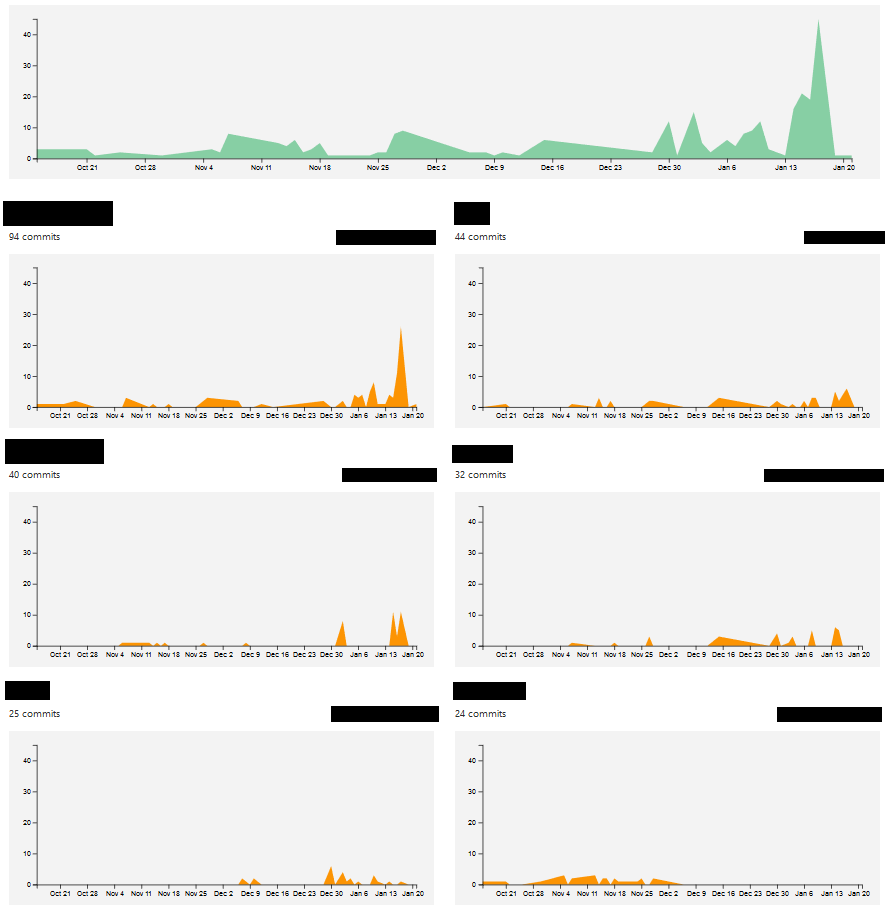
\includegraphics[scale=0.4]{slike/aktivnost.PNG} %veličina slike u odnosu na originalnu datoteku i pozicija slike
			\centering
			\caption{Primjer slike s potpisom}
			\label{fig:promjene}
		\end{figure}
		
		\begin{figure}[H]
			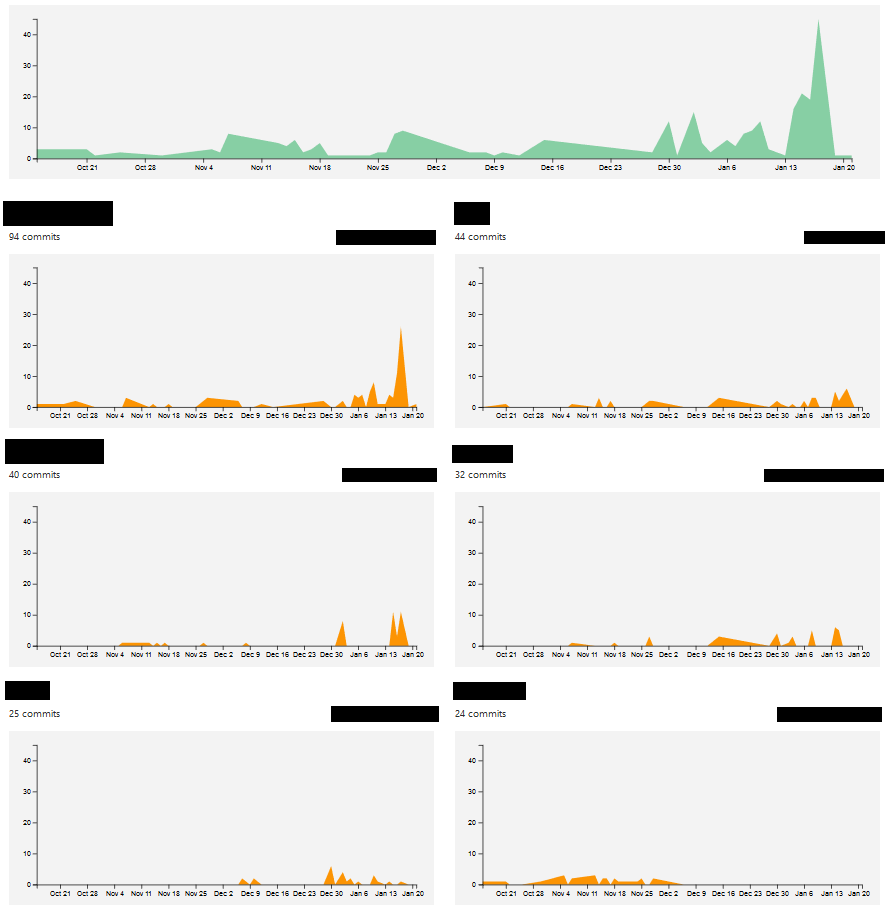
\includegraphics[width=\textwidth]{slike/aktivnost.PNG} %veličina u odnosu na širinu linije
			\caption{Primjer slike s potpisom 2}
			\label{fig:promjene2} %label mora biti drugaciji za svaku sliku
		\end{figure}
		
		Referenciranje slike \ref{fig:promjene2} u tekstu.
		
		\eject
		
	